\subsubsection{Windows terminal}

Windows Terminal is a pretty new tool released from Microsoft in which you can do a lot of customizations such as:

\begin{itemize}
    \item Use tabs for the same or different distributions
    \item Change colors
    \item Fast start SSH to server through Ubuntu
    \item And much more...
\end{itemize}

\subsubsubsection{Installing}

In order to continuously get updates, install winget by going to the \link{https://github.com/microsoft/winget-cli/releases/}{Microsoft Github page} and downloading a file called something like:

\code{Microsoft.DesktopAppInstaller_8wekyb3d8bbwe.msixbundle}

Execute the file and install/update.

Thereafter, open up \code{cmd} and enter winget to verify that it is accessible.

Open \code{cmd} and install Windows Terminal with:

\code{winget install --id=Microsoft.WindowsTerminal -e}

\subsubsubsection{Custom colors}

You are able to customize your colors in Windows terminal through a \code{.json} file. It is recommended setting Visual Studio Code as your standard \code{.json} file viewer as it shows a small color sample of every \code{#rrggbb} color.

Open Windows Terminal, and press \code{Ctrl + ,}. Then at the far bottom left corner, click \textbf{Open JSON file}.

Here you can add custom schemes and do other settings. I recommend using my custom color scheme by copy and appending this to your schemes:

\begin{minted}{text}
{
    "name": "Solarized Dark Custom",
    "background": "#002B36",
    "black": "#002B36",
    "blue": "#FFFFFF",
    "brightBlack": "#073642",
    "brightBlue": "#747D7D",
    "brightCyan": "#93A1A1",
    "brightGreen": "#00A0FF",
    "brightPurple": "#6C71C4",
    "brightRed": "#CB4B16",
    "brightWhite": "#FDF6E3",
    "brightYellow": "#657B83",
    "cursorColor": "#FFFFFF",
    "cyan": "#2AA198",
    "foreground": "#A8A8A8",
    "green": "#056E32",
    "purple": "#D33682",
    "red": "#DC322F",
    "selectionBackground": "#FFFFFF",
    "white": "#EEE8D5",
    "yellow": "#B58900" 
},
\end{minted}

Then, within the \code{json} file, go to profiles and look for your Ubuntu distribution.

\begin{figure}[H]
    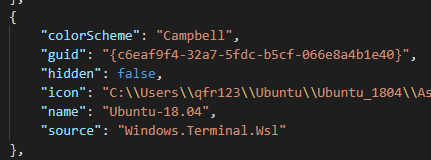
\includegraphics[width=0.55\textwidth]{figures/json_1.PNG}
\end{figure}

Change \code{"colorScheme"} to \code{"Solarized Dark Custom"}

\begin{figure}[H]
    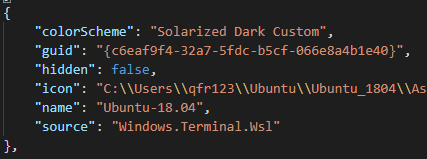
\includegraphics[width=0.55\textwidth]{figures/json_2.PNG}
\end{figure}

\subsubsubsection{Set your distro as default}

Open the settings \code{.json} file through \code{Ctrl + c} then pressing \textbf{Open JSON file} far bottom left.

You can choose the default distribution to be opened up when opening Windows Terminal.

Change \code{<guid>} in \code{"defaultProfile": <guid>} to the one corresponding to the profile with your distribution.

\begin{figure}[H]
    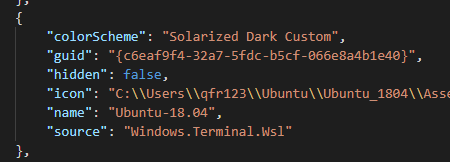
\includegraphics[width=0.55\textwidth]{figures/json_3.PNG}
\end{figure}

\textbf{Default location}

Also, one might want Ubuntu to open up at a specific location such as the Ubuntu home folder.

In Ubuntu:

\code{cd ~ && explorer.exe .}

Copy the path and add the key

\code{"startingDirectory": <path>}

and replace the path. For every \code{\ } you will need to add another \code{\ } in order for windows to understand.

\mintinline{text}{\\\\wsl$\\Ubuntu-18.04\\home\\<username>}

\subsubsubsection{Profile for SSH through distribution}

In Windows Terminal, open up the settings with \code{Ctrl + ,}.

Press \textbf{+ Add a new profile} and chose your distribution to duplicate. Press \textbf{Duplicate}:

\begin{center}
    \resizebox{0.95\textwidth}{!}{%
        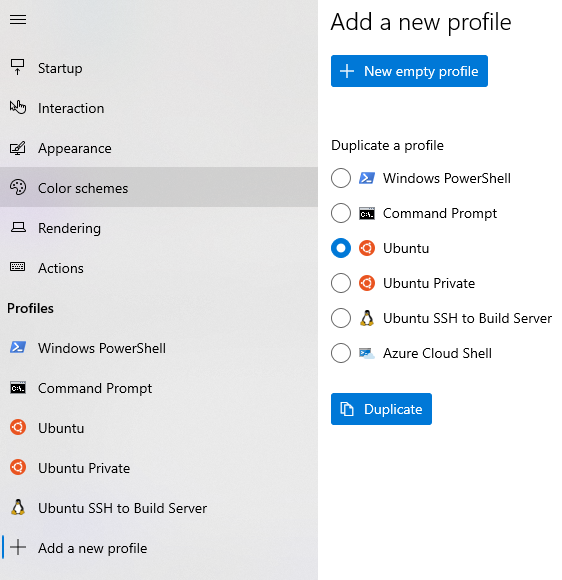
\includegraphics[height=5cm]{figures/duplicate_distro_1.PNG}
        \,
        \vrule
        \,
        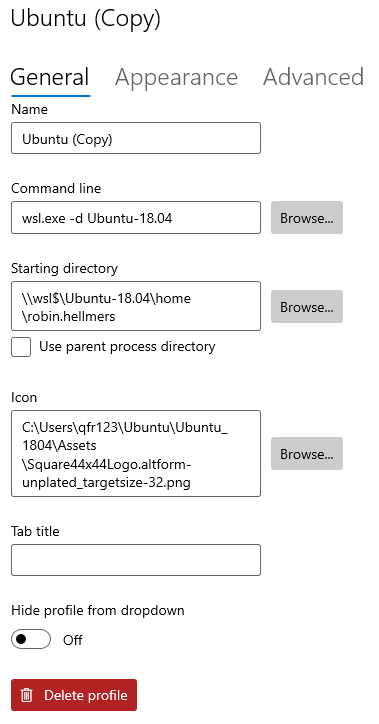
\includegraphics[height=5cm]{figures/duplicate_distro_2.PNG}
    }
\end{center}

Give the new name e.g. \textit{Ubuntu SSH to Server}.

At the field \textbf{Command line}, append

\code{ssh <username>@<IP address server>}

or if your have a password for the server username

\code{ssh-pass -p <password> ssh <username>@<IP address server>}

so it looks something like 

\code{wsl.exe -d Ubuntu-18.04 ssh <username>@<IP address server>}

or

\code{wsl.exe -d Ubuntu-18.04 ssh-pass -p <password> ssh <username>@<IP address server>}.

Then \textbf{Save} it.

Now press the newly added profile and see if you can SSH into the server.

\begin{figure}[H]
    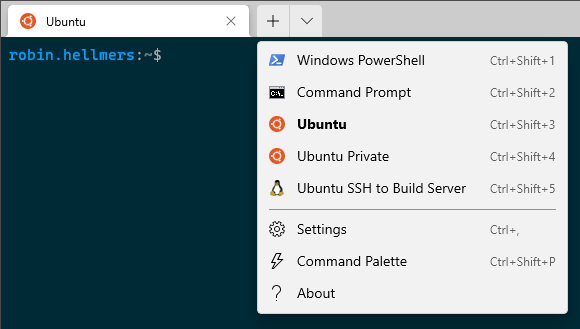
\includegraphics[width=0.7\textwidth]{figures/profiles_dropdown.PNG}
\end{figure}

If it prompts you for your password. Open up at normal Ubuntu window and enter

\code{ssh-copy-id <username>@<IP address build server>}

and enter your password. Now try to SSH again.

